\subsection{Neural Networks}
A human brain is composed of billions of neurons, connected and excitable cells which allow humans to be intelligent. Each neuron's dendrites receive signals from other neurons. If the these electrical signals exceed a threshold, the neuron fires, thereby propagating a voltage out of its synapses and on to other neurons. Together, these neurons form an extensive network, where an immense set of sensory input i processed alongside expected outputs. The purpose of artificial neural networks is to simulate this same network of interconnected neurons using mathematical properties to emulate electrical signals and approximate complex functions
\subsubsection{Artificial Neurons}
\input{Sections/Diagrams/Neuron.tex}
An artificial neuron is an approximate mathematical model of a biological neuron, and is intended to fulfill similar purposes. Each artificial neuron has multiple inputs from other neurons. Along with the inputs, each neuron has a weight for each input, a bias term, and activation function, and only one output. The output of one neuron travels to other neurons and becomes of their inputs. The output of a neuron is expressed mathematically for $n$ inputs $x$ and weights $w$, a bias term $b$, and activation function $f(x)$ as follows:

$$activation = \sum\limits_{i=0}^n x_i w_i+b$$
$$output = f(activation)$$


Mentioned above, weights are positive or negative numbers which scale the effect or relevance of their accompanying inputs on a neuron's single output. Besides the weights, another important component of a neuron is the activation function, whose primary is to transform the output of a neuron. Common activation functions include a sigmoid curve, a hyperbolic tangent, a binary step function, and a rectifier function.The sigmoid activation and hyperbolic tangent activation functions are often used for general purpose neural networks due to their gradient nature, fixed range, and the fact that they are easily differentiated. Finally, the bias term is a number added to the summation of weighted inputs, which allows us to make transformations on the domain of the activation function.
\begin{figure}[h]
\centering
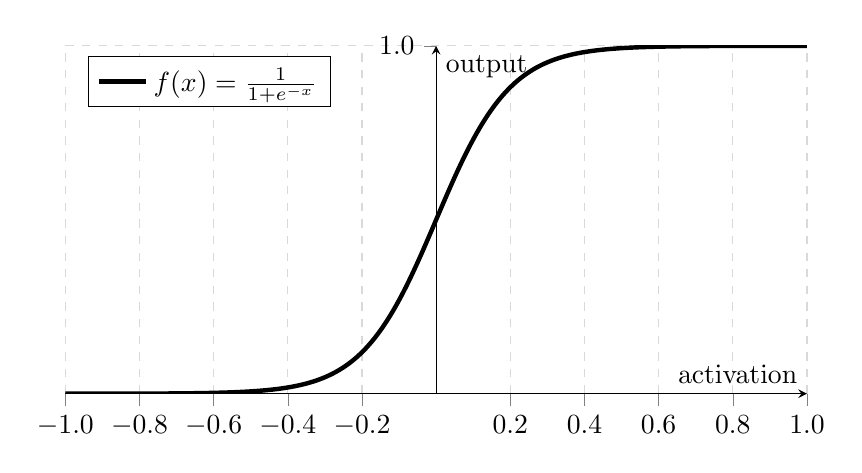
\begin{tikzpicture}
    \begin{axis}[
    	legend pos=north west,
        axis x line=middle,
        axis y line=middle,
        ytick={0,1},
        x tick label style={/pgf/number format/fixed,
                            /pgf/number format/fixed zerofill,
                            /pgf/number format/precision=1},
        y tick label style={/pgf/number format/fixed,
                            /pgf/number format/fixed zerofill,
                            /pgf/number format/precision=1},
        grid = major,
        width=11cm,
        height=6cm,
        grid style={dashed, gray!30},
        xmin=-1,     % start the diagram at this x-coordinate
        xmax= 1,    % end   the diagram at this x-coordinate
        ymin= 0,     % start the diagram at this y-coordinate
        ymax= 1,   % end   the diagram at this y-coordinate
        %axis background/.style={fill=white},
        xlabel=activation,
        ylabel=output,
        tick align=outside,
        enlargelimits=false]
      % plot the stirling-formulae
      \addplot[domain=-1:1, black, ultra thick,samples=500] {1/(1+e^(-10*x))};
      \addlegendentry{$f(x)=\frac{1}{1+e^{-x}}$}
    \end{axis}
\end{tikzpicture}
\caption{Sigmoid Function Graph}
\end{figure}
\subsubsection{Feed-forward Neural Network}
Constellation utilizes a feed-forward neural network, a collection of neurons organized into layers, as classifying mechanism for detection various features in a image. In a feed-forward neural network, the output of each neuron is the input of each neuron in the next layer. In this manner, the original inputs of the network are "fed forward" to new neurons in new layers, passing through a number of hidden layers in the middle, and finishing at the output layer.The outputs of the neurons in the final layer (output layer) are the outputs of the whole network and are used to judge the conclusion the network made.